% ----- formatovani dokumentu -----------------------------------------------
\documentclass[12pt,a4paper,titlepage,final]{report}
\usepackage[utf8]{inputenc}
\usepackage[T1, IL2]{fontenc}
\usepackage{graphicx}
\usepackage{epstopdf}
\usepackage[margin=2cm]{caption}
\usepackage[top=3cm, left=2cm, right=2cm, text={17cm, 24cm}, ignorefoot]{geometry}
\usepackage[usenames,dvipsnames]{color}
\usepackage[]{algorithm2e}
\usepackage{amsmath}

% ------ commands -----------------------


% ---------------------------------------

\usepackage{url}
\usepackage{setspace}
\singlespacing
\usepackage[square, numbers]{natbib} 
\pagestyle{plain}
\pagenumbering{arabic}
\setcounter{page}{1}

\setlength{\parindent}{1cm}	
\usepackage{natbib}
\renewcommand{\thesection}{\arabic{section}}
\renewcommand{\thesubsection}{\arabic{section}.\arabic{subsection}}



% ----- vyberte jazyk -------------------------------------------------------
\usepackage[english,czech]{babel}
%\usepackage[english]{babel}

% ----- dopiste titulky -----------------------------------------------------
\newcommand\Course{Počítačové vidění}
\newcommand\WorkTitle{Detekce objektů na CUDA, jejich rozpoznávání a sledování}
\newcommand\AuthorA{Pavel Macenauer}
\newcommand\AuthorB{Jan Bureš}
\newcommand\AuthorAEmail{xmacen02@stud.fit.vutbr.cz}
\newcommand\AuthorBEmail{xbures19@stud.fit.vutbr.cz}
\newcommand\Faculty{Fakulta Informačních Technologií}
\newcommand\School{Vysoké Učení Technické v~Brně}

\usepackage[
pdftitle={\WorkTitle},
pdfauthor={\AuthorA\AuthorB},
bookmarks=true,
colorlinks=true,
breaklinks=true,
urlcolor=blue,
citecolor=blue,
linkcolor=blue,
unicode=true,
]
{hyperref}



% ----- titulni strana ------------------------------------------------------

\begin{document}
	\begin{titlepage}
	\begin{center}
		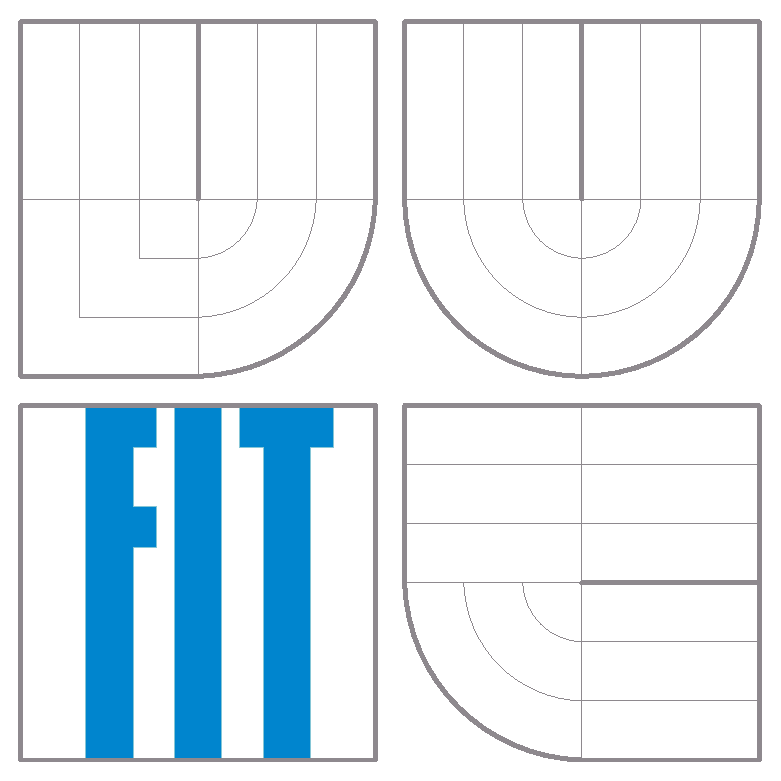
\includegraphics[height=5cm]{images/logo.eps}
	\end{center}
	\vfill
	\begin{center}
		\begin{Large}
			\Course\\
		\end{Large}
		\bigskip
		\begin{Huge}
			\WorkTitle\\
		\end{Huge}
	\end{center}
	\vfill
	\begin{center}
		\begin{large}
			\today
		\end{large}
	\end{center}
	\vfill
	\begin{flushleft}
		\begin{large}
			\begin{tabular}{lll}
				Autor: & \AuthorA, & \url{\AuthorAEmail} \\
				& \AuthorB, & \url{\AuthorBEmail} \\
		
				& & \\
				& \Faculty \\
				& \School \\
			\end{tabular}
		\end{large}
	\end{flushleft}
\end{titlepage}		

\tableofcontents

% ----- obsah -------------------------------------------------------------
\newpage

\section{Cíl práce}

Cílem této práce je naimplementovat detektor objektů na GPU pomocí technologie NVidia CUDA a následně i rozšíření pro rozpoznání obličeje a jeho sledování. Vstupem jsou obrazová data (fotografie, video) a výstupem obrazová data a statistiky s vyznačenými detekcemi odpovídající sledovaným/detekovaným objektům.

\section{Detekce objektů}

Detektor objektů ke svému běhu používá 2 typy algoritmů. 

\begin{itemize}
	\item Metalgoritmus, který zpracovává celý průběh detekce, tedy skládá jednotlivé slabé klasifikátory v jeden silný a nakonec prohlásí, zda-li se jedná nebo nejedná o hledaný objekt – \textbf{Waldboost}
	\item 	Algoritmus pro vyhodnocení slabého klasifikátoru – \textbf{LBP} (Local Binary Patterns)
	\end{itemize}

\subsection{Waldboost}
Jak již bylo zmíněno výše, Waldboost je metalgoritmus, který skládá slabé klasifikátory v jeden silný. Vychází z metalgoritmu Adaboost s tím rozdílem, že v každém svém kroku kontroluje, zda-li akumulovaná odezva nepřesáhla určitou mez. V případě, že ano, zařadí jej do odpovídající třídy, jinak pokračuje vyhodnocování dále. Dojede-li na konec, zkontroluje ještě konečnou mez a následně vrátí výsledek. Formálně lze popsat následovně:

\begin{algorithm}
\KwData{$h^{(t)}$, $\theta_{A}^{(t)}$, $\theta_{B}^{(t)}$, $\gamma$, $x$}
\KwResult{+1, -1}
\Begin{
\For{$1$ \KwTo $T$}{
	\If{$H_{T}\geq\theta_{B}^{(t)}$}{
	 	classify x to the class +1 and terminate
	 }
	\If{$H_{T}\leq\theta_{A}^{(t)}$}{ 
		classify x to the class -1 and terminate
	}
}


\eIf{$H_{T}>\gamma$}
{classify x to the class +1}
{classify x to the class -1}
 }
\caption{Algoritmus WaldBoost}
\end{algorithm}

\subsection{LBP příznaky}
Konkrétní odezva slabého klasifikátoru je závislá na použitých příznacích. Detektor používá příznaků LBP (Local Binary Patterns).

\begin{figure}[ht]
\begin{center}
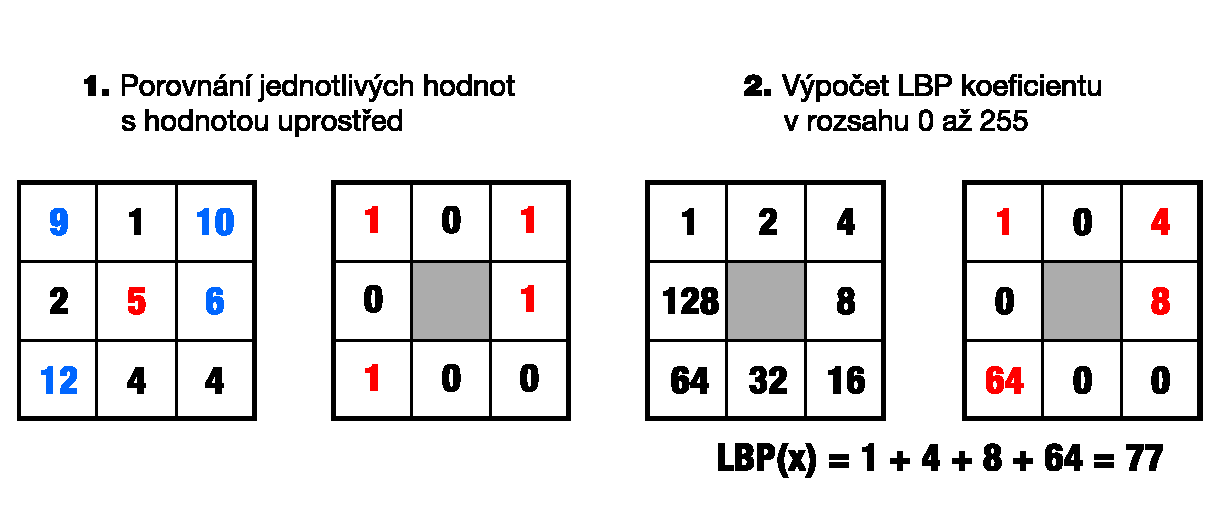
\includegraphics[width=14cm]{images/lbp.eps}
\caption{Výpočet LBP příznaku}
\label{fig:theory}
\end{center}
\end{figure}

\section{Implementace detektoru na GPU}
GPU se oproti CPU liší především tím, že obsahuje mnohonásobně více výpočetních jader. Není vhodné tedy zpracovávat data sekvenčně, kdy by se jedním jádrem, kterých můžou být v případě moderních grafických karet stovky až tisíce, zpracovával celý výpočet, ale paralelně, kdy využijeme všech.

Detektor má 2 základní fáze:
\begin{itemize}
	\item Vytvoření pyramidového obrazu
	\item Detekce obličejů na pyramidovém obrazu
\end{itemize}

\subsection{Vytvoření pyramidového obrazu}
Vláken se rozeběhne tolik, kolik je pixelů původního obrazu. Následně se z každého pixelu vytváří zmenšeniny.

Jednotlivé zmenšeniny se vytvářejí po oktávách a úrovních. V jednoduchosti lze říci, že zmenšeniny jsou omezeny na maximální a minimální velikost. Vytvoří tolik obrazů kolik je oktáv * úrovní a nevytvářejí se již zmenšeniny, které jsou menší, než určitá mez.
Každé vlákno vezme tedy jeden pixel původního obrazu a sekvenčně prochází jednotlivé zmenšeniny dané mírou zmenšení a v nich ho umísťuje.

Výstupem je jeden obraz, ve kterém jsou jednotlivé zmenšeniny původního obrazu. Tento obraz se následně nabinduje jako textura.

\subsection{Detekce objektů}
Vstupem do samotné detekce je pyramidový obraz uložený jako textura. Vláken se rozeběhne tolik, kolik je pixelů pyramidového obrazu.

Každý pixel je počátkem vzorku daného velikostí, na kterou je natrénován detektor. V našem případě 26x26. Následně prochází jednotlivými stages detektoru a snižuje nebo zvyšuje odezvu. V případě, že odezva spadne pod mez danou konkrétní stagí, je výpočet pro daný vzorek ukončen. V případě, že výpočet projde přes všechny stages, je zkontrolována ještě konečná mez, na odstranění parazitních vzorků s velmi malou odezvou. Pokud je odezva větší i než konečná mez, jedná se o hledaný objekt.

Takovýchto detekcí je tradičně více na jednom místě a to pro jednotlivé zmenšeniny.

\subsection{Uspořádání paměti}
Podstatné součásti detektoru jsou rozděleny na následující části. Typy paměti jsou dle názvosloví CUDA :

\begin{itemize}
\item \textbf{Stages} – constant memory \\
	K jednotlivým stages je přistupováno sekvenčně pro každý pixel (výpočetní vlákno) obrazu. Jsou tak broadcastováný do všech výpočetních jader.
\item \textbf{Alphas} – texture (global) memory \\
	Náhodné přístupy do constant memory by dělali přístup k alphám velmi neefektivní, protože by se zbytečně broadcastovaly. Navíc se jedná o data, kterých je více, než-li constant memory na většině grafických karet. Texturovací pamět je optimalizována pro náhodný read-only přístup.
	
\item \textbf{Původní obraz} – texture (global) memory
	Texturovací pamět, krom toho, že je optimalizována pro náhodné read-only přístupy umožňuje bilineární interpolaci 2D dat. Lze tak za pomocí hardwarových jednotek počítat zmenšeniny obrazu
	
\item \textbf{Pyramidový obraz} – texture (global) memory

\item \textbf{Obrazové parametry} – constant memory \\
	Parametry obrazu, se kterými se hojně pracuje, např. velikost obrazu jsou taktéž ukládány v constant memory. Vzhledem k tomu, že se pro jednotlivá vlákna nemění, je vhodné je broadcastovat a využívat rychlého přístupu.
\end{itemize}
	
\section{Trackování a rozpoznávání obličejů}

Jak bylo uvedeno výše, detektor zpravidla vrací více detekcí na jednom místě pro jednotlivé zmenšeniny. Proto se při trackování nejprve z těchto mnoha detekcí vybere oblast, kde se obličej nalézá. Tento výpočet probíhá tak, že se prochází jednotlivé detekce a zkoumá se, zda nepřekrývají nějakou jinou alespoň z 50\%. Pokud ano vybere se detekce s lepší odezvou, jinak není oblast do trackování obličejů zahrnuta.

Celá oblast se poté převede do barevného modelu HSV (Huge, Saturation, Value), který lépe poslouží pro rozpoznávání podobností mezi obličeji. Samotné porovnání se provádí pomocí histogramu vytvořeného na základě obrázku v barevném modelu HSV, kde pro výpočet histogramu postačí pouze hodnoty H a S. Hodnotu V jsme se rozhodli vypustit z důvodu proměnlivých podmínek osvětlení obličeje, například při pohybu člověka od/ke zdroji osvětlení scény (lampa, okno, \dots). 

K výpočtu rozdílnosti histogramu jsme využili metodu zvanou „Bhattacharyya distance“ viz. následující vzorec:

\begin{figure}

\begin{align}
d(H_{1},H_{2})=\sqrt{1-\frac{1}{\sqrt{\overline{H_{1}}\overline{H_{2}}N^2}}\sum\limits_{I}\sqrt{H_{1}(I) \cdot H_{2}(I)}}
\end{align}

\caption{Bhattacharyya distance}
\end{figure}



				
Pomocí tohoto vzorce zjistíme rozdílnost histogramu v rozsahu hodnot $<0;1>$ (0 - stejné histogramy, 1 - histogramy nemají nic společného). 

K porovnání dvou obličejů jsme využili víše uvedený postup při porovnání histogramu obličeje, ke kterému jsme ještě přidali vzdálenost oblasti, na které se obličej nacházel při posledním výskytu ve videu (popřípadě v sekvenci obrázků). Předpokládáme, že v sekvenci obrázku se daný obličej nebude přesouvat skokově, neboli vzdálenost od posledního výskytu bude u jednoho obličeje velmi malá. Problém by mohl nastat, pokud se obličej vytratí ze záběru a objeví se později v jiné jeho části (například odchod z místnosti a pozdější návrat jiným vchodem). Z toho důvodu jsme se rozhodli normalizovat vzdálenost do rozmezí $<0;0,5>$ a přičíst k hodnotě rozdílnosti histogramu. Na základě součtu hodnocení se pak prochází uložené obličeje a vybere se nejlepší shoda. Pokud hodnocení nepřesáhne daný práh (nastaven na 0,6) prohlásí se obličej za shodný s dříve rozpoznaným. V opačném případě je obličej přidán do seznamu obličejů jako unikátní.

\section{Rozdělení práce}
\paragraph{Pavel Macenauer} detektor objektů na GPU (zároveň diplomová práce), rozpoznání objektů a kostra aplikace

\paragraph{Jan Bureš} sledování objektů a jejich rozpoznávání, výstupy z aplikace

\section{Ovládání programu}

\subsection{Překlad}

\begin{itemize}
\item Závislost na knihovnách: OpenCV 2.4.* (testováno na 2.4.9, 2.4.10), CUDA 6.5 \\

\item Pro vlastní překlad je třeba stáhnout obsah repositáře, kde je přiložen projekt pro Microsoft Visual Studio 2013 a mít nainstalované výše zmíněné závislosti, popř. ve složce \verb|final\bin| je spustitelný balíček pro Windows:\\  \url{https://github.com/mmaci/vutbr-fit-pov-face-tracking}
\end{itemize}


\subsection{Spuštění}

Program se spouští přes příkazovou řádku s následujícími parametry: \\
\verb|-ii [input file] or -di [dataset] or| \\ \verb|-iv [input video] and -ot [output track info]|

\begin{itemize}
\item \textbf{Input file} – vstupní obrázek
\item \textbf{Dataset} – textový soubor obsahující seznam obrázků
\item \textbf{Input video} – vstupní video
\item \textbf{Output track info} – soubor pro textový výstup
\end{itemize}

Výstupem je textový soubor s výsledky trackování a výřezy jednotlivých obličejů. Vše je uloženo ve stejné složce, ve které je spuštěna aplikace.

\begin{figure}[ht]
\begin{center}
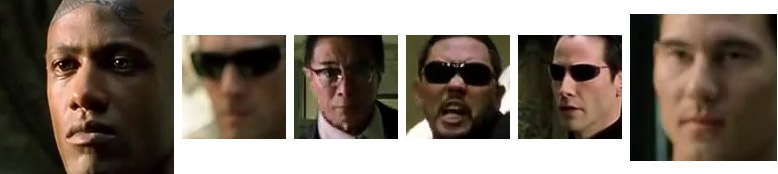
\includegraphics[width=14cm]{images/faces.jpg}
\caption{Příklady detekovaných obličejů}
\label{fig:theory}
\end{center}
\end{figure}

\begin{figure}[ht]
\begin{center}
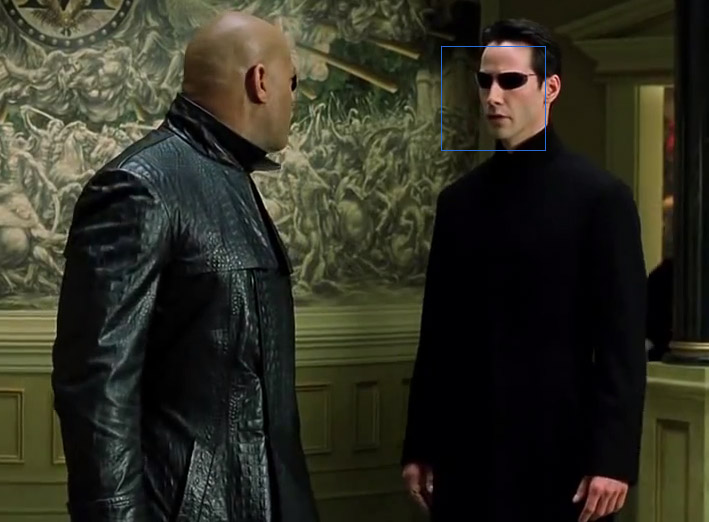
\includegraphics[width=14cm]{images/matrix.jpg}
\caption{Ukázka výstupu na videu}
\label{fig:theory}
\end{center}
\end{figure}

\section{Závěr a vize do budoucnosti}

Naimplementovaný detektor objektů je funkční a na mobilní grafické kartě Nvidia Quadro K1000M zvládá detekovat obličeje na HD obraze průměrně za 100ms, což odpovídá 10 FPS. Na zvýšení rychlosti by bylo třeba omezit výpočet např. zredukováním počtu vyhodnocovaných stagí z 2048 na 1/2 nebo 1/4, čímž snížíme jeho přesnost, ale snížíme délku výpočtu pod úroveň FPS v běžných videích.

Výpočetní náročnost trackování obličejů je vzhledem k detektoru zanedbatelná. Pro porovnání obličeje je využit histogram oblasti, na které se obličej nachází a vzdálenost mezi současnou a předchozí pozicí obličeje. Zkoušeli jsme i porovnání na základě extrakce klíčových bodů, ale tento způsob nevykazoval dobré výsledky.

\vspace{0.5cm}
\noindent Další možné optimalizace do budoucnosti jsou:

\paragraph{Zpřesnění generování zmenšenin}
Aktuálně jsou sice generovány z texturovací paměti, ale v ní jsou uložena obrazová data jako unsigned char, což vede ke zmenšeninám pomocí alg. Nearest neighbour. Převod na float by umožnil bilineární interpolaci pomocí hardwaru.
	
\paragraph{Rozdělení vyhodnocování stagí na více kernelů a reorganizace vláken}
Aktuálně probíhá vyhodnocování stagí od začátku do konce v rámci jednoho kernelu. Většina vzorků je však zamítnuta již na začátku. Šlo by tak zjistit, pro které vzorky stále ještě běží výpočet a spustit nový kernel pouze pro ně.
	
\paragraph{Optimalizace zmenšenin na velikost videa} 
Velikost videa je často standardizována na velikost a poměr stran (16:9, 4:3, HD, FULL HD, …). Šlo by tak generovat zmenšeniny pro daný standard, kde by se využilo maximum obrazové plochy, zmenšila její velikost a výpočet by šlo urychlit rozbalením cyklů.

\paragraph{Optimalizace rozpoznání obličejů}
Do budoucna bychom chtěli přidat další možnosti porovnání obličejů, protože v současnosti je velká váha přiložena právě vzdálenosti mezi předchozí a současnou pozicí obličeje.



\bibliographystyle{plain}

\nocite{cite1}
\nocite{cite2}
\nocite{cite3}
\nocite{cite4}


\hypertarget{bib}{}
\bibliography{reference}
\addcontentsline{toc}{section}{Literatura}

\end{document}

